%\vspace{-2cm}

\chapter*{Introduction}
\addcontentsline{toc}{chapter}{Introduction} % serve per inserire l'Indice nel Table of contents

Silicon detectors represent a cornerstone technology in particle physics experimentation. Their predominant application lies in tracking systems designed to precisely reconstruct the trajectories of charged particles. Additionally, they function as active sensing elements within sampling calorimeters for specific experimental configurations. This calorimetric application is anticipated to gain significance due to the growing demand for high-granularity calorimeters essential for particle flow reconstruction methodologies \cite{krammer2015silicon}.

In this project, the characteristics of a silicon strip sensor and its readout electronics are examined with a Educational Alibava System (EASy) \cite{EASY}, through systematic irradiation using two distinct sources.
Initial calibration employs a laser source to establish baseline detector response under controlled, well-defined conditions. Subsequently, a radioactive isotope replaces the laser to emulate realistic detection scenarios. The selected isotope, strontium-90 ($^{90}\mathrm{Sr}$), undergoes $\beta⁻$ decay, producing yttrium-90 ($^{90}\mathrm{Y}$) as a daughter nucleus. This $^{90}\mathrm{Y}$ isotope itself decays via $\beta⁻$ emission to stable zirconium-90 ($^{90}\mathrm{Zr}$), forming a two-stage decay chain. \autoref{fig:decayChain} details this sequence, including the half-lives ($T_{1/2}$) of both isotopes and the maximum kinetic energies ($\beta_{1,\mathrm{max}}$, $\beta_{2,\mathrm{max}}$) of the emitted electrons.

\begin{figure}[H]
       %\setkeys{Gin}{draft=false}
	\centering
	\fcolorbox{black}{white}{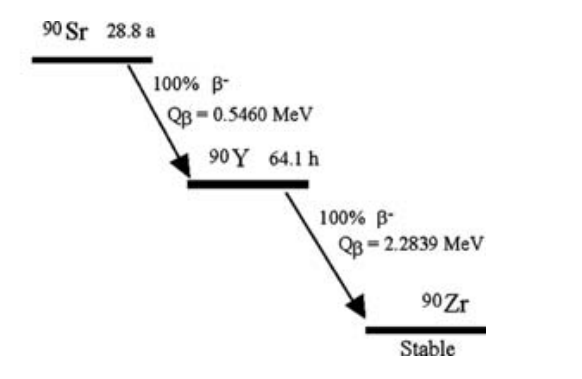
\includegraphics[scale=0.4]{pictures/decayChain.png}}
	\caption{Decay chain of the isotope 90 Sr, from \cite{attrep2008determination}.}
	\label{fig:decayChain}
\end{figure}

As both decay stages generate electron emissions, their energy spectra are recorded concurrently. The substantial separation between the characteristic endpoint energies of the $^{90}\mathrm{Sr}$ and $^{90}\mathrm{Y}$ decays allows for clear spectroscopic discrimination and independent analysis of the two electron distributions.
